\section{Metodologia}
\subsection{Selezione delle feature}\label{subsec:feature_selection}
Innanzitutto, è stato individuato un sottoinsieme delle feature presenti in EMBER, con l'obiettivo di ridurre i tempi di addestramento delle reti, mantenendo al contempo elevate prestazioni in termini di accuratezza.\newpage
\end{multicols}

\begin{figure}[t]
\centering
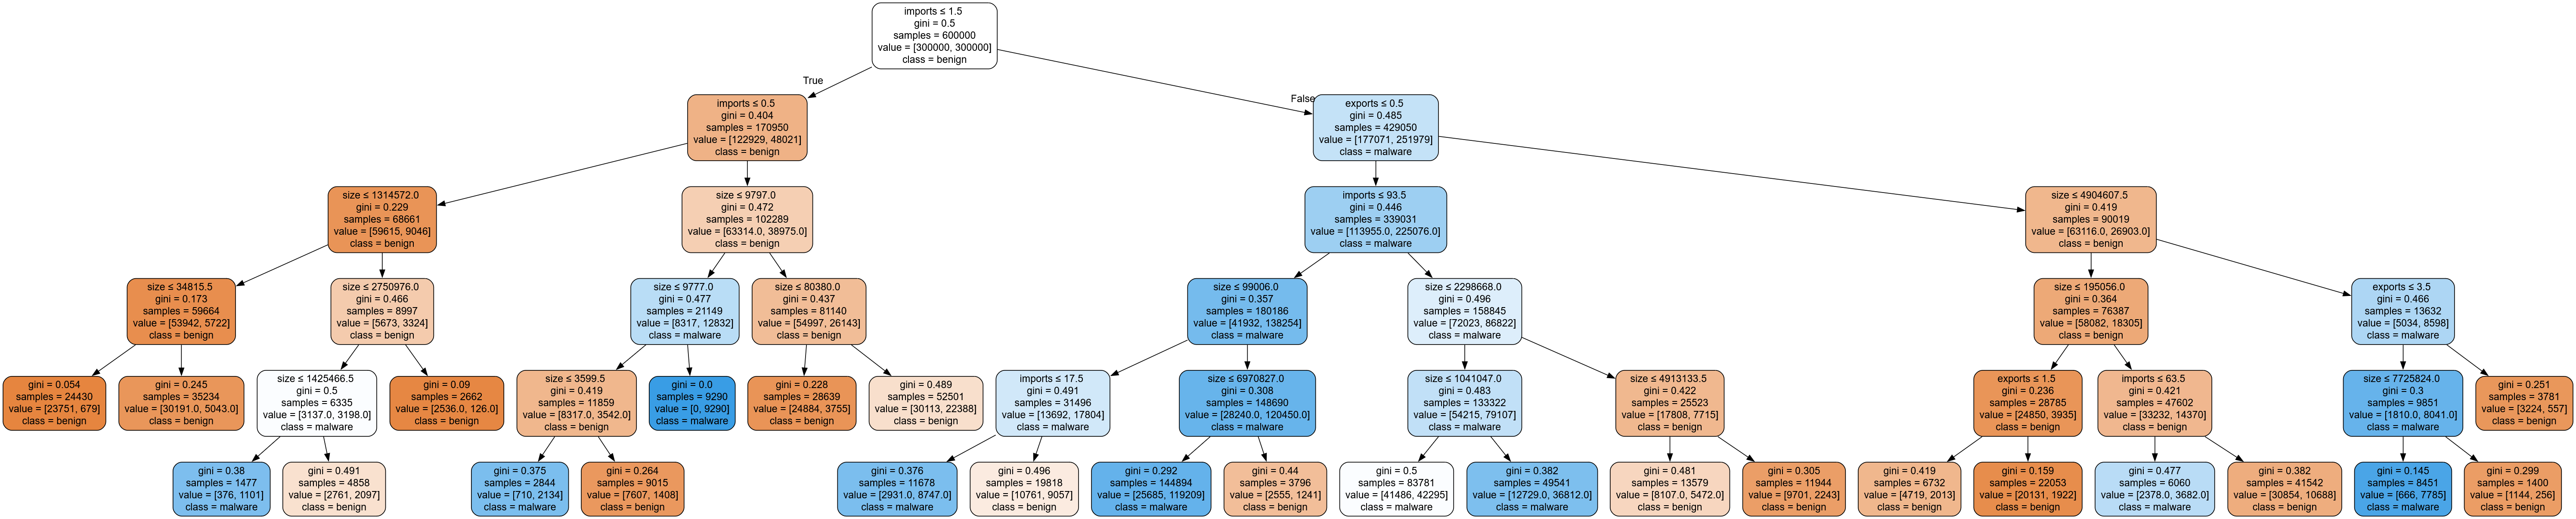
\includegraphics[width=\textwidth]{fig/decision_tree.png}
\caption{Esempio di albero di decisione semplificato tramite pruning} 
\label{fig:decision_tree}
\end{figure}

\begin{multicols}{2}
Poiché il progetto mira a sviluppare un sistema interpretabile, particolare attenzione è stata riservata alle feature con un significato facilmente comprensibile per un essere umano. Le feature selezionate provengono dalle categorie \textbf{General} e \textbf{Header}, per un totale di 23 feature.

\subsection{Estrazione delle regole}
Dopo aver selezionato le feature di interesse, sono state generate tutte le possibili combinazioni di tre feature, ottenendo un totale di 1540 combinazioni. Ogni combinazione è stata utilizzata per addestrare e testare un albero di decisione (il \textbf{rule learner}). Successivamente, è stato applicato un processo di pruning su ciascun albero per migliorare la capacità di generalizzazione del modello e ridurre la complessità strutturale dell'albero. In Figura~\ref{fig:decision_tree} è riportato un esempio di albero di decisione semplificato tramite pruning. Le regole decisionali sono state estratte da ogni albero che, durante la fase di test, ha raggiunto un'accuratezza pari o superiore al 70\%. Di seguito è riportato un esempio di queste regole:
\begin{lstlisting}
|--- imports <= 1.50
|   |--- imports <= 0.50
|   |   |--- size <= 1314572.00
|   |   |   |--- size <= 34815.50
|   |   |   |   |--- weights: [23751.00, 679.00] class: 0.0
|   |   |   |--- size >  34815.50
|   |   |   |   |--- weights: [30191.00, 5043.00] class: 0.0
|   |   |--- size >  1314572.00
|   |   |   |--- size <= 2750976.00
|   |   |   |   |--- size <= 1425466.50
|   |   |   |   |   |--- weights: [376.00, 1101.00] class: 1.0
|   |   |   |   |--- size >  1425466.50
|   |   |   |   |   |--- weights: [2761.00, 2097.00] class: 0.0
|   |   |   |--- size >  2750976.00
|   |   |   |   |--- weights: [2536.00, 126.00] class: 0.0
...
\end{lstlisting}
In particolare, ogni foglia del tipo 
\smallskip
\begin{lstlisting}
weights: [23751.00, 679.00] class: 0.0
\end{lstlisting}
serve a determinare le informazioni associate a un nodo specifico dell'albero decisionale. I valori indicati come \texttt{weights} rappresentano il numero di campioni del dataset che ricadono in quel nodo per ciascuna classe. Nell'esempio mostrato, 2536.00 campioni appartengono alla classe 0 (quella dei file benigni) e 126.00 all'altra (malware). Il valore di \texttt{class} (0.0) indica la classe predetta per quel nodo, tipicamente determinata in base alla maggioranza dei campioni associati.
\newline\newline
Tra i 1540 alberi addestrati, 133 hanno superato la soglia di accuratezza del 70\% durante la fase di test.
\subsection{Creazione delle regole ASP}\label{subsec:asp_rules}
Ciascuno dei 133 file contenenti le regole estratte dagli alberi migliori è stato analizzato mediante espressioni regolari, con l'obiettivo di generare le corrispondenti regole ASP. Nello specifico, la testa di ogni regola ASP include un letterale nella forma:  
\begin{verbatim}class(V)\end{verbatim}  
dove \texttt{class} può essere \texttt{benign\_score} o \texttt{malign\_score}, a seconda della classe predetta, e \texttt{V} rappresenta il peso associato alla classe, come definito nella Sezione~\ref{subsec:decision_tree}. Il corpo della regola è costituito da una sequenza di coppie di letterali nella forma:  
\begin{verbatim}feature(X), X cond Y\end{verbatim}  
Qui, \texttt{feature} corrisponde a una caratteristica estratta nella Sezione~\ref{subsec:feature_selection}, mentre \texttt{cond Y} rappresenta la condizione derivata da uno degli alberi di decisione addestrati. Ad esempio, riprendendo l'esempio precedente, ogni regola assume una struttura simile alla seguente:  
\begin{lstlisting}
benign_score(23751) :- 
imports(Z), Z <= 15, 
imports(Y), Y <= 5, 
size(X), X <= 13145720, 
size(W), W <= 348155.
\end{lstlisting}  
Le regole estratte, in totale 2436, sono state quindi aggregate e costituiscono la parte intensionale del programma ASP che verrà utilizzato per la rilevazione dei malware. Si noti che, poiché ASP non consente di operare con valori decimali, si è reso necessario eseguire una trasformazione dei dati, scalando i valori di ciascuna feature di un fattore pari a 10. In questo modo, tutti i valori numerici sono stati convertiti in numeri interi.

Per calcolare il punteggio totale associato alle classi \texttt{benign\_score} e \texttt{malware\_score}, sono state inserite le regole
\begin{lstlisting}
benign_total(S) :- 
S = #sum { V : benign_score(V) }. 

malware_total(S) :-
S = #sum { V : malware_score(V) }.
\end{lstlisting}

che sfruttano l'operatore aggregato \texttt{\#sum} per sommare tutti i pesi di una determinata classe e assegnarli alle variabili \texttt{BS} e \texttt{MS}. E

\begin{lstlisting}
benign :-
benign_total(BS), malware_total(MS), BS >= MS. 
	
malware :- 
benign_total(BS), malware_total(MS), MS > BS. 
\end{lstlisting}
con cui deriviamo \texttt{benign} o \texttt{malware} confrontando i valori di tali variabili.

\subsection{Definizione dei fatti ASP}
Per definire la parte estensionale del programma, è necessario inserire una serie di fatti di tipo
\begin{lstlisting}
feature(V).
\end{lstlisting}  
dove \texttt{feature} è, ancora una volta, una delle caratteristiche estratte nella Sezione~\ref{subsec:feature_selection} e \texttt{V} rappresenta il valore della feature per il campione da classificare, moltiplicato per un fattore di scala di 10. Ad esempio, \texttt{imports(15).} indica che il valore della feature \texttt{imports} è pari a 15. In questo modo, per ciascun campione del set di dati vengono generati i fatti ASP corrispondenti, ai quali vengono poi aggiunte le regole ASP precedentemente definite. Infine, attraverso l’utilizzo del modulo \texttt{clingo} di Python \cite{clingo_api}, si procede alla classificazione del programma, determinando se il campione in esame debba essere etichettato come benigno o come malware.